
This section provides a formal model of the problem described with Alloy modeling language. 
The model considers the most important constraints. In addition to the model there are some 
possible worlds meant to clarify some critical aspects.
Simplifications: 

\subsection{Alloy model}
\lstinputlisting[language=alloy]{alloy_model.als}

\subsection{First World}
In the first world (Figure \ref{fig:world1}) the focus is on the registration of some farmers. Because we assume that they uses the application for the first time, the only information present are the ones required for the registration. Email and username are unique, not like password and surname that could be the same for different farmers (but them does not exist without an associated user). 
Because each farmer is associated to a farm we only create a world with 3 farm and it automatically generate the same amount of different farm as well. We also did not generate any Policy Maker to highlight the possibility of the farmers only to registered



\subsection{Second World}
The second world showed in (Figure \ref{fig:world2}) focuses on a single farm with multiple evaluations. Therefore it is considered a farm, with his owner and all their characteristics. Every evaluation made on the farm has a different date, more precisely it does not have the same month, a different messageContent. They are written by different policy makers but the most important thing to notice is that the receiver of the evaluation is the same owner of the farm that has the evaluations.


\subsection{Third World}
The third world (Figure \ref{fig:world3}) highlight the possibility to the farmers to comunicate to each other throw the forum sending messages and the report by a farmer of a production he made in his farm in a specific date. Each message send in the forum have exactly  one sender (a farmer only) and is verified that the sender can write one message at a time.  The forum is unique but it can be empty (look at world 1) if no-one has send any message yet. On the other side each production submitted in a day must be of different type in a farm, because it has the field ‘quantity’ to specify the amount so is not necessary to generate a Production for each harvest.

\begin{sidewaysfigure}
    \begin{center}
          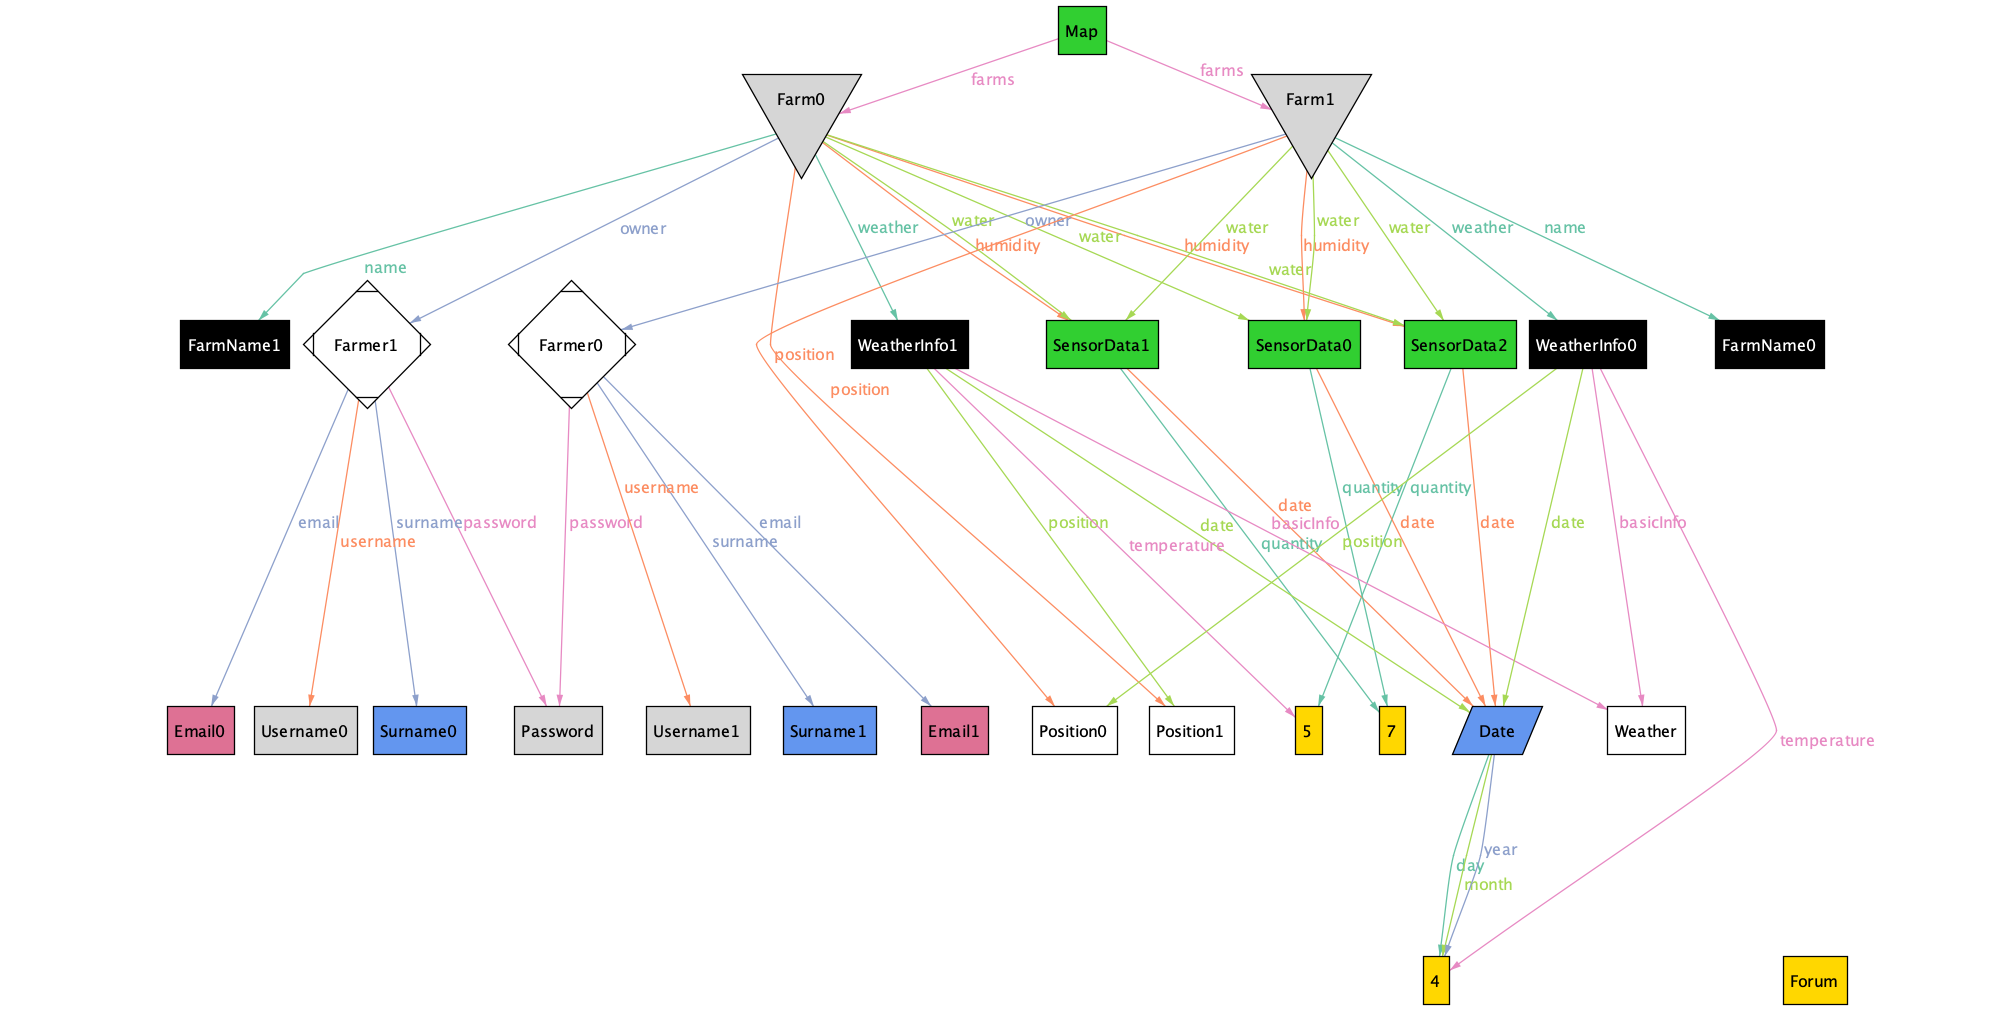
\includegraphics[width=1.2\textwidth]{alloy/world1.png}
          \caption{FirstWorld}
        \label{fig:world1}
    \end{center}
\end{sidewaysfigure}


\begin{sidewaysfigure}
    \begin{center}
          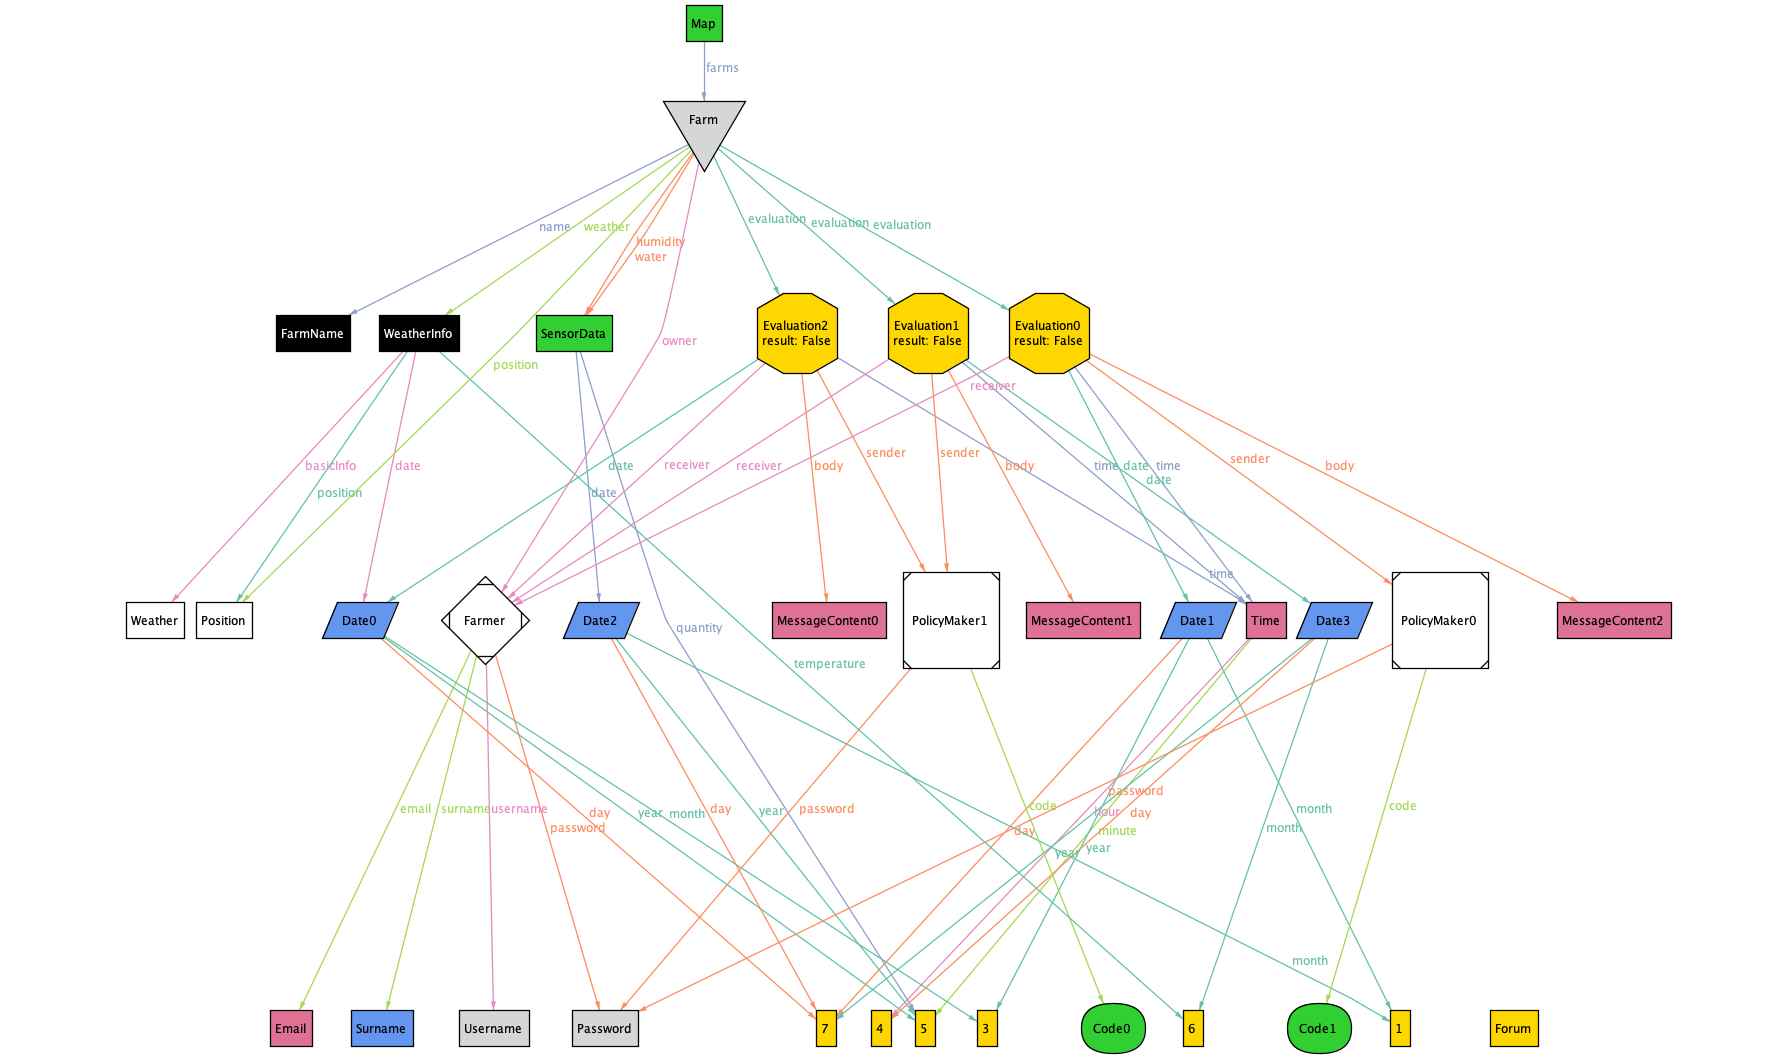
\includegraphics[width=1.2\textwidth]{alloy/world2.png}
          \caption{Second World}
        \label{fig:world2}
    \end{center}
\end{sidewaysfigure}

\begin{sidewaysfigure}
    \begin{center}
          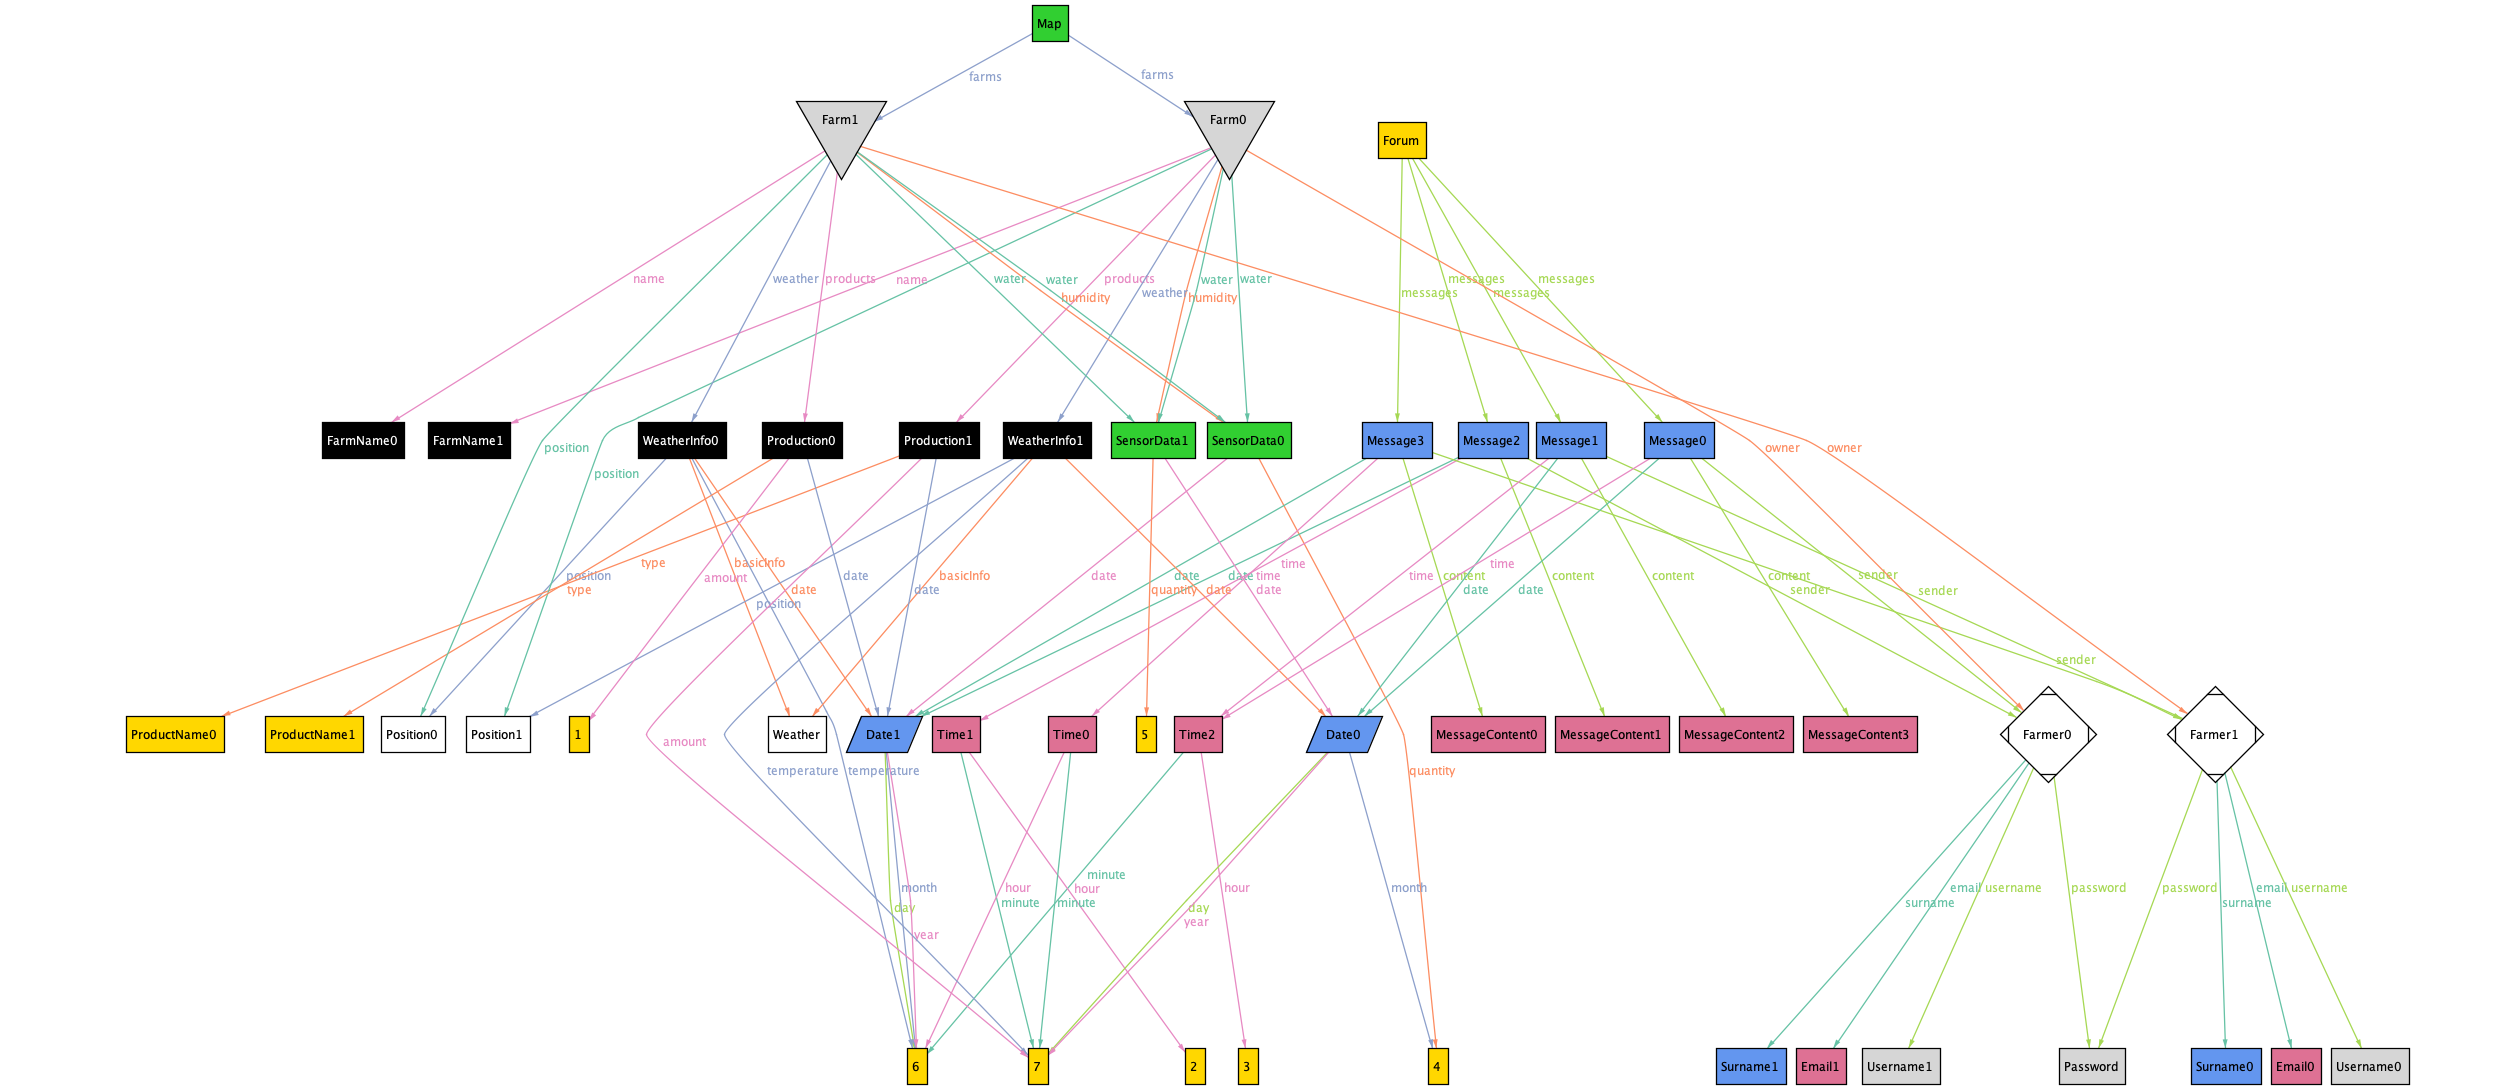
\includegraphics[width=1.2\textwidth]{alloy/world3.png}
          \caption{Third World}
        \label{fig:world3}
    \end{center}
\end{sidewaysfigure}

